This document contains the mathematical details for constructing a smooth spline through a data set.
In addition to fitting the data, the spline should be smooth (jerk-minimizing) and satisfy known boundary conditions precisely.
The resulting spline can be generated by solving a linear system ($x = A \backslash b$).

\begin{figure}[ht]
	\centering
  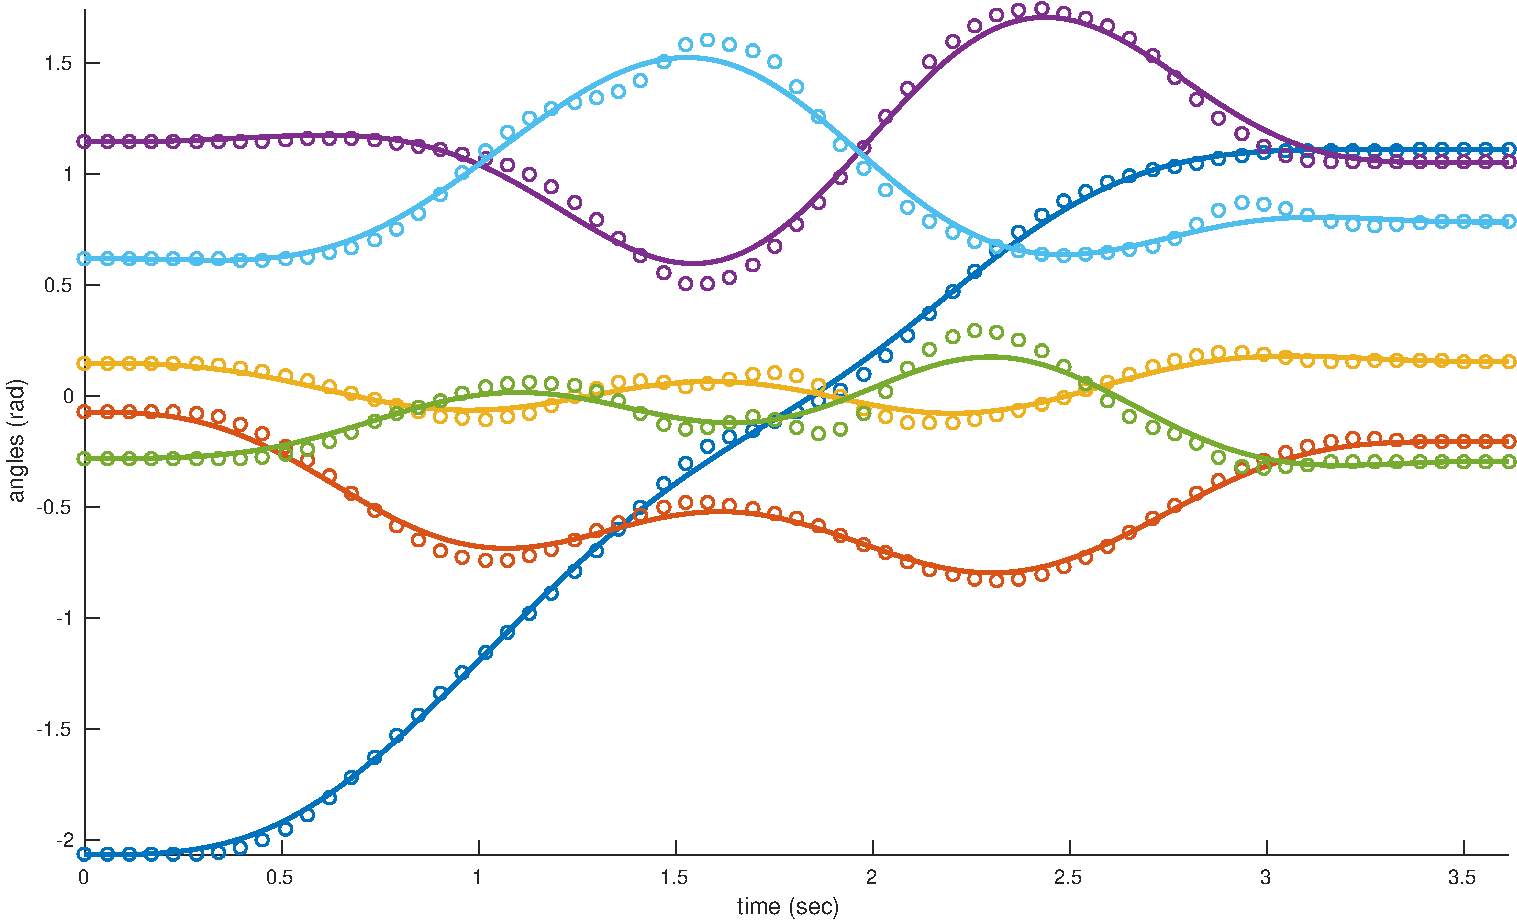
\includegraphics[width=\textwidth]{fig/DataFittingExampleFigure.pdf}
  \caption{A spline that is fit to a six-dimensional data set, trading off between data-fitting and
           minimizing jerk. The slope and curvature at the start and end are set to zero.}
  \label{fig:DataFittingExampleFigure}
\end{figure}

\newpage
